\chapter{Herramienta Web. \emph{Front-End}}
\label{frontend}
Nuestra aplicación Web esta dividida en \emph{back-end} y \emph{front-end}. En el capítulo anterior se describió el \emph{back-end}. El propósito de
este capítulo es describir el \emph{front-end}. El \emph{front-end} es el encargado de la capa de presentación.
\par
El \emph{front-end} es implementado en JavaScript\cite{JavaScript}. Este es un lenguaje de programación soportado por la mayoría de navegadores Web,
nos permite dotar de funcionalidad extendida a nuestras páginas Web. Actualmente el uso de este lenguaje esta tan extendido y avanzado que permite
crear aplicaciones enteras para navegadores Web. Existen múltiples frameworks escritos en JavaScript que facilitan la creación de aplicaciones Web. En
este trabajo vamos a utilizar dos, Sencha ExtJs\cite{ExtJs} y HighStock\cite{HighStock}.
\par
Sencha ExtJs es un framework orientado a la creación de aplicaciones Web interactivas. Debido al gran abanico de funcionalidades que este framework
presenta, podemos decir que este es de propósito general. Este ofrece abstracciones para gestionar nuestros datos, arquitectura MVC, componentes
gráficos de control y otros.
\par
HighStock es un framewrok con un propósito específico. Este está orientado a facilitar la creación de gráficos. El framework es muy eficiente, esto
reduce la carga computacional de nuestra aplicación. Los gráficos generados por este son altamente interactivos, permiten ocultar series, navegar,
realizar zoom y mucho más
\par
Como podemos ver en la figura \ref{fig:frontend} nuestro \emph{front-end} esta basado en el patrón de diseño 
\emph{modelo-vista-controlador}\cite{MVCWiki}.
\begin{figure}[h]
	\centering
	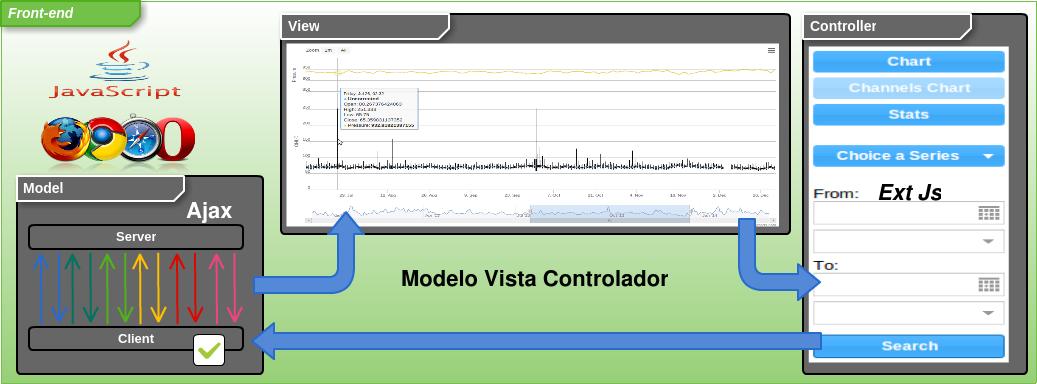
\includegraphics[keepaspectratio, width=1\textwidth]{./img/frontend.png}
	\caption{\emph{Front-end}. Patrón MVC.}   
	\label{fig:frontend}
\end{figure}

